\section{Laboratory work implementation}

\subsection{Tasks and Points}

\begin{itemize}
	\item initializeaza un nou repositoriu
	\item configureaza-ti VCS
	\item crearea branch-urilor (creeaza cel putin 2 branches)
	\item commit pe ambele branch-uri (cel putin 1 commit per branch)
	\item seteaza un branch to track a remote origin pe care vei putea sa faci push (ex. Github, Bitbucket or custom server)
	\item reseteaza un branch la commit-ul anterior
	\item folosirea fisierului .gitignore
	\item merge 2 branches
	\item rezolvarea conflictelor a 2 branches
	\item folosirea tag-urilor pentru marcarea schimbarilor simnificative precum release-ul.
\end{itemize}

\subsection{Analiza lucrarii de laborator}
Repository \href{https://github.com/AScripnic/MIDPS-laboratories/tree/master/Lab%231}{link}

Primul pas a fost crearea unui nou repositoriu prin intermediul UI-ului oferit de github, iar mai precis apasând pe butonul \hl{New} de pe pagina utilizatorului, tab-ul cu denumirea \hl{Repositories}. După setarea numelui pentru repositoriu, am apăsat \hl{create repository}.

Al doilea pas a constituit în crearea unui ssh key și l-am copiat în lista mea de key in account-ul github, ce mi-a permis editarea datelor din repositoriul creat anterior \cite{ssh}. Apoi am clonat repositoriul local prin intermediul la instrucțiunea: git clone git@github.com:AScripnic/MIDPS-laboratories.git .

Mi-am configurat config-ul la git cli prin intermediul la intrucțiunile git config user.name "ascripnic" și git config user.email "scripnic.alexandru@gmail.com" \cite{set-config}.

În al treilea pas am create 2 branchuri și câte un commit în fiecare (referintă: \ref{2-branches})prin intermediul comenzii \hl{git branch} și denumirea branch-ului de care am avut nevoie și \hl{git commit -am} și mesajul commitului. Este și posibilitatea de a crea și a te muta pe branchul create printr-o commandă \hl{git checkout -b}. Cu ajutorul comenzii  \hl{git push origin} și denumirea la branch am încărcat schimbarile pe remote origin.

În al patrulea pas am resetat un branch, după ce am adăugat un fișier nou și i-am făcut commit,la commit-ul anterior (referință: \ref{revert}) cu ajutorul comenzii \hl{git reset HEAD\~} \cite{reset}.

În al cincilea pas am adăugat un fișier în .gitignore (referință: \ref{ignore}) ce a făcut comenzile git să nu îl considere ca un fișier din proiect, cu excepția unor comenzi ce forțează git cli să lucreze cu acest fișier.

În al șaselea pas am făcut merge la 2 branchuri (referință: \ref{merge}) cu ajutorul comenzii \hl{git merge} și denumirea la branch-ul cu care aș dori să fac merge \cite{merge}.

În al șaselea pas am creat un conflict între 2 branchuri, schimbând același fișier apoi am făcut \hl{git pull} unul din altul, ce a generat un conflict (referință: \ref{conflict-appear}). Sunt mai multe metode de a fixa un conflict, unele din ele ar fi:
\begin{itemize}
	\item Manual - selectarea manuală a informației care trebuie sa rămână, și ștergerea celei inutile sau care nu mai este necesară
	\item Cu ajutorul comenzii \hl{git checkout [--theirs|--ours]} ce ar preoretiza schimbările în dependență de alegerea făcută \cite{checkout-fix}. 
	\item Cu ajutorul unor tool-uri care sunt prezente în unele IDE
\end{itemize} 

Eu am ales varianta manuală (referință: \ref{fixed}) și o prefer mai mult ca a 2-a variantă pentru a înlătura riscurile de pierdere de date. Apoi am făcut commit cu fixarea făcută (referință: \ref{resolvedcommit}).

Pentru ultimul pas am creat un \href{https://github.com/AScripnic/MIDPS-laboratories/releases/tag/v0.0.1}{tag nou} (referință: \ref{release}) cu ajutorul butonului \hl{Draft a new release} de pe pagina \url{https://github.com/AScripnic/MIDPS-laboratories/releases}.

\subsection{Imagini}
\begin{center}
	\begin{figure}[h]
		\centering
		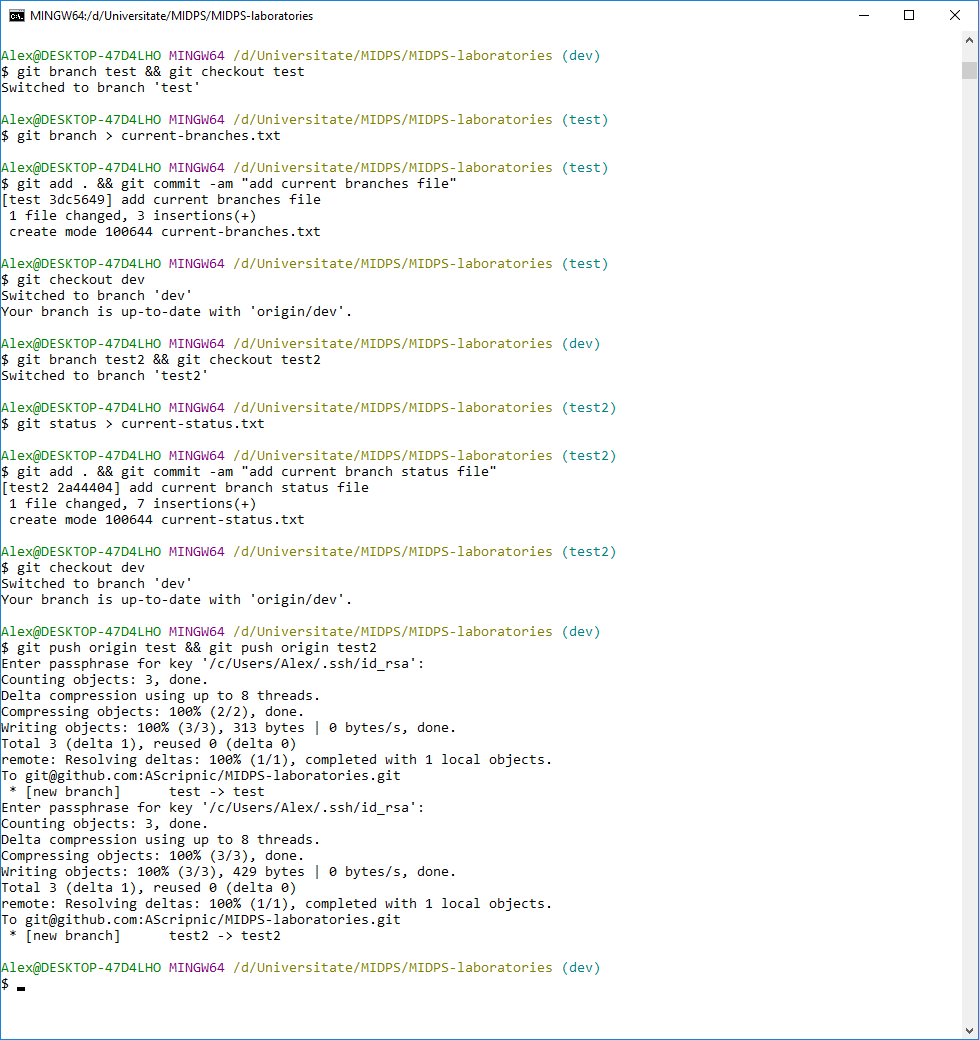
\includegraphics[width=15cm]{2-branches}\\
		\caption{Adaugarea a 2 branch-uri și câte un commit}
		\label{2-branches}
	\end{figure}
	\begin{figure}[h]
		\centering
		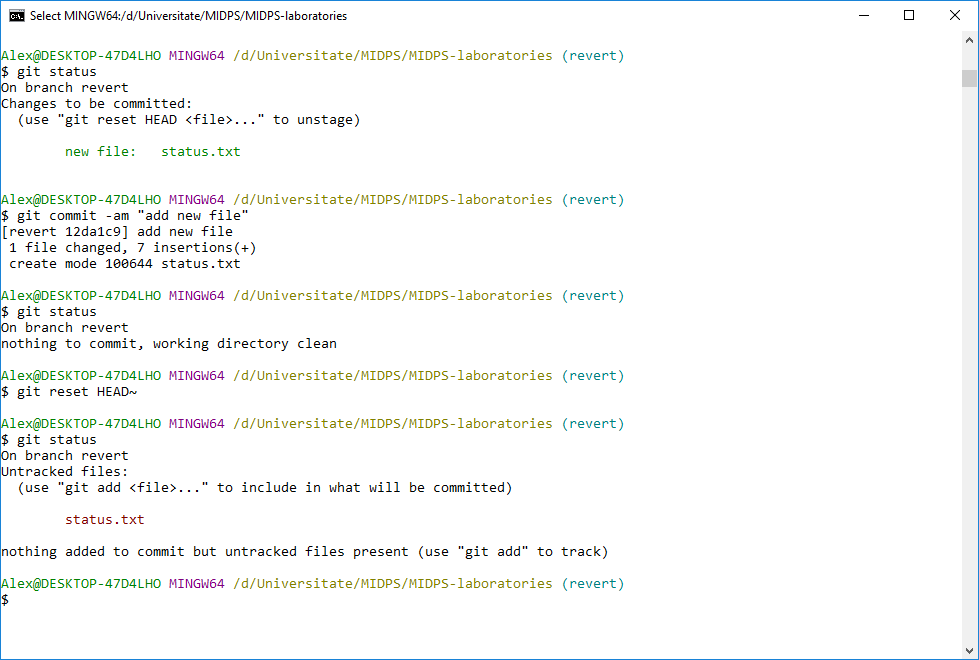
\includegraphics[width=15cm]{revert}\\
		\caption{Reset la commit anterior}
		\label{revert}
	\end{figure}
	\begin{figure}[h]
		\centering
		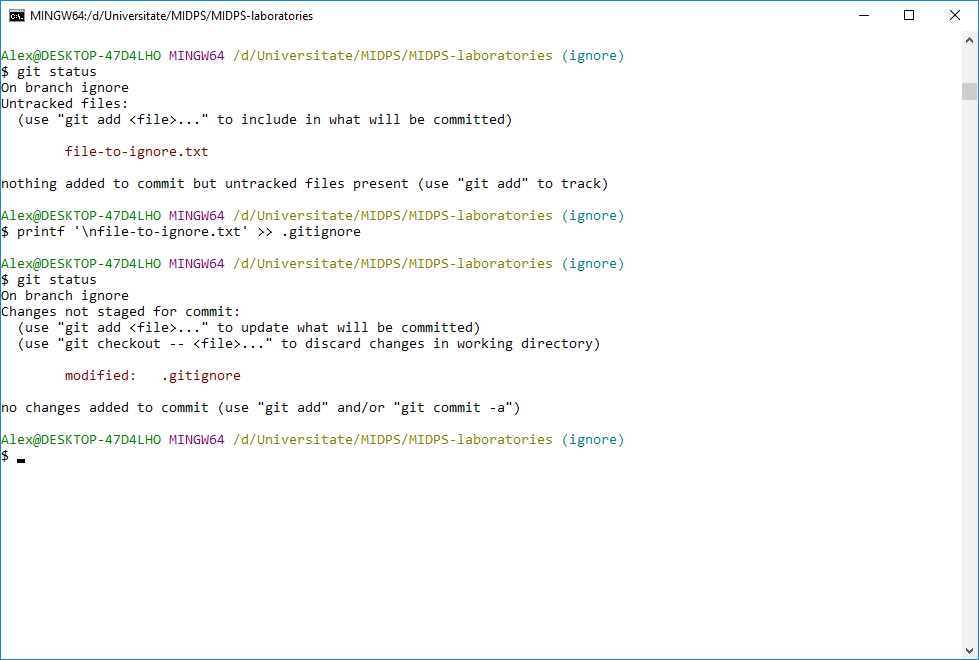
\includegraphics[width=15cm]{ignore}\\
		\caption{Adăugarea unui fișier în .gitignore}
		\label{ignore}
	\end{figure}
	\begin{figure}[h]
		\centering
		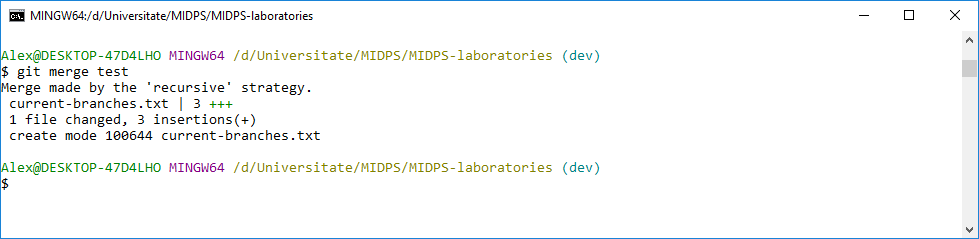
\includegraphics[width=15cm]{merge}\\
		\caption{Merge la 2 branch-uri}
		\label{merge}
	\end{figure}
	\begin{figure}[h]
		\centering
		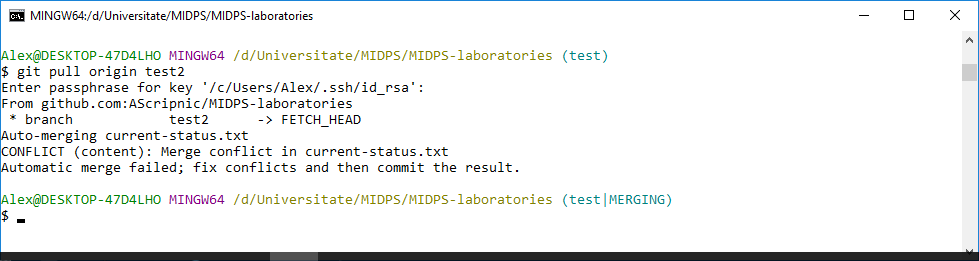
\includegraphics[width=15cm]{conflict-appear}\\
		\caption{Crearea unui conflict}
		\label{conflict-appear}
	\end{figure}
	\begin{figure}[h]
		\centering
		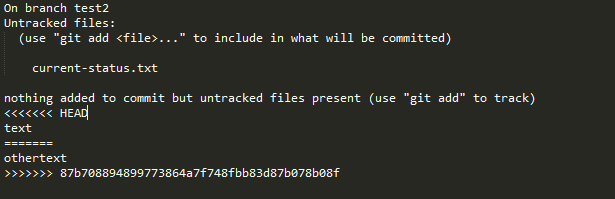
\includegraphics[width=15cm]{conflicted}\\
		\caption{Fișierul în care a avut loc conflictul}
		\label{conflicted}
	\end{figure}
	\begin{figure}[h]
		\centering
		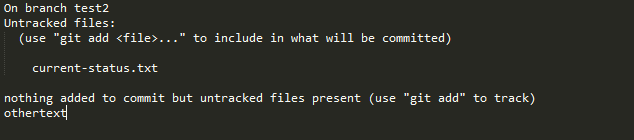
\includegraphics[width=15cm]{fixed}\\
		\caption{Fișierul fixat după conflict}
		\label{fixed}
	\end{figure}
	\begin{figure}[h]
		\centering
		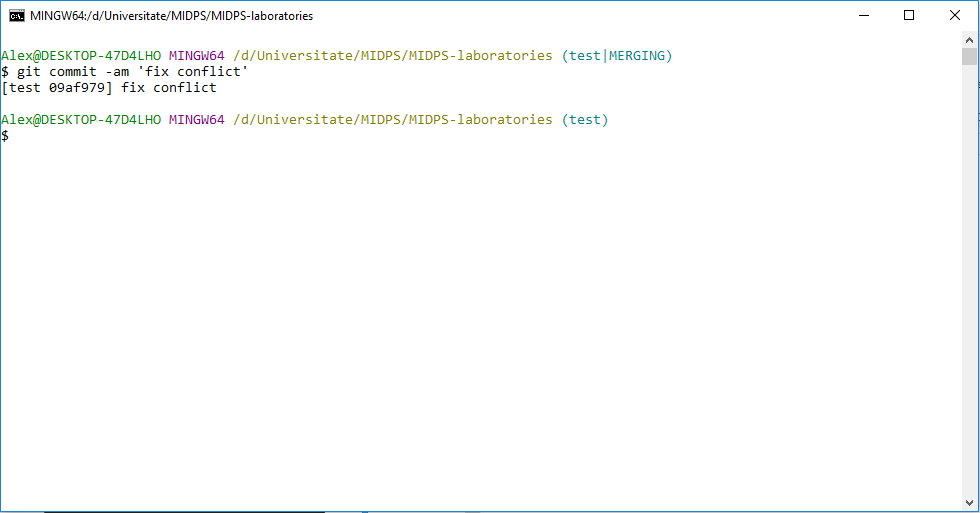
\includegraphics[width=15cm]{resolvedcommit}\\
		\caption{Commit după rezolvarea conflictelor}
		\label{resolvedcommit}
	\end{figure}
	\begin{figure}[h]
		\centering
		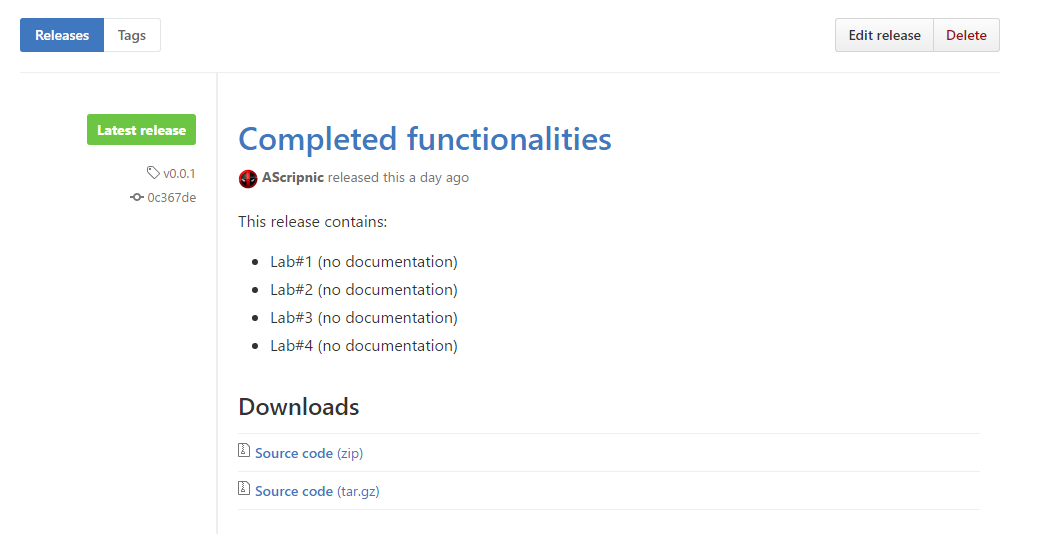
\includegraphics[width=15cm]{release}\\
		\caption{Crearea unui tag nou}
		\label{release}
	\end{figure}
\end{center}

\clearpage
